\chapter{Introduction}

Population geneticist are historians telling the story of evolution. Mutation and recombination leave faithful historical records in the genome of every single organism on earth. The records have always been there, but over the past decades, the experimental and computational tools to decipher those records have improved dramatically. This introductory chapter surveys several key methodological trends that have transformed population genetic research, and finally delineates how these trends have built up the momentum for the original work presented in this thesis.

\section{Genealogical modeling of evolution using the \acl{ARG}} \label{intro-arg}

%% Intro from pedigree to ARG, explain coalescence and recombination
The genetic relationships between ancestors and descendants form the basis of all evolutionary genomics research. The simplest data structure that encodes ancestor-descendant relationships is a pedigree (light grey in Fig. \ref{fig:intro-F1}A), commonly known as a ``family tree". The pedigree is a graphical structure representing genealogical ancestry of individual organisms. During meiosis in sexually-reproducing diploid organisms, any given position in a haploid gamete is randomly sampled from either chromosome through meiotic recombination. Consequently, the pedigree alone cannot fully specify the genetic ancestry of every position in the genome. Since random shuffling of parental chromosomes through recombination creates a mosaic of genetic ancestry along the genome, different non-recombining segments of the genome have different paths of genetic inheritance in the pedigree. The collection of all paths (or lineages) along which inherited segments of the genome have been transmitted forms a complex graphical structure embedded in the pedigree known as an \acf{ARG} (dark grey in Fig. \ref{fig:intro-F1}A, \cite{griffiths1997progress}). The \ac{ARG} is a \textit{complete} record of the history of genetic inheritance for a set of sampled genomes (solid nodes \textcircled{A}, \textcircled{B}, \textcircled{C} and \textcircled{D} at the tips of the \ac{ARG} in Fig. \ref{fig:intro-F1}).

\begin{figure}%[h]
    \centering
    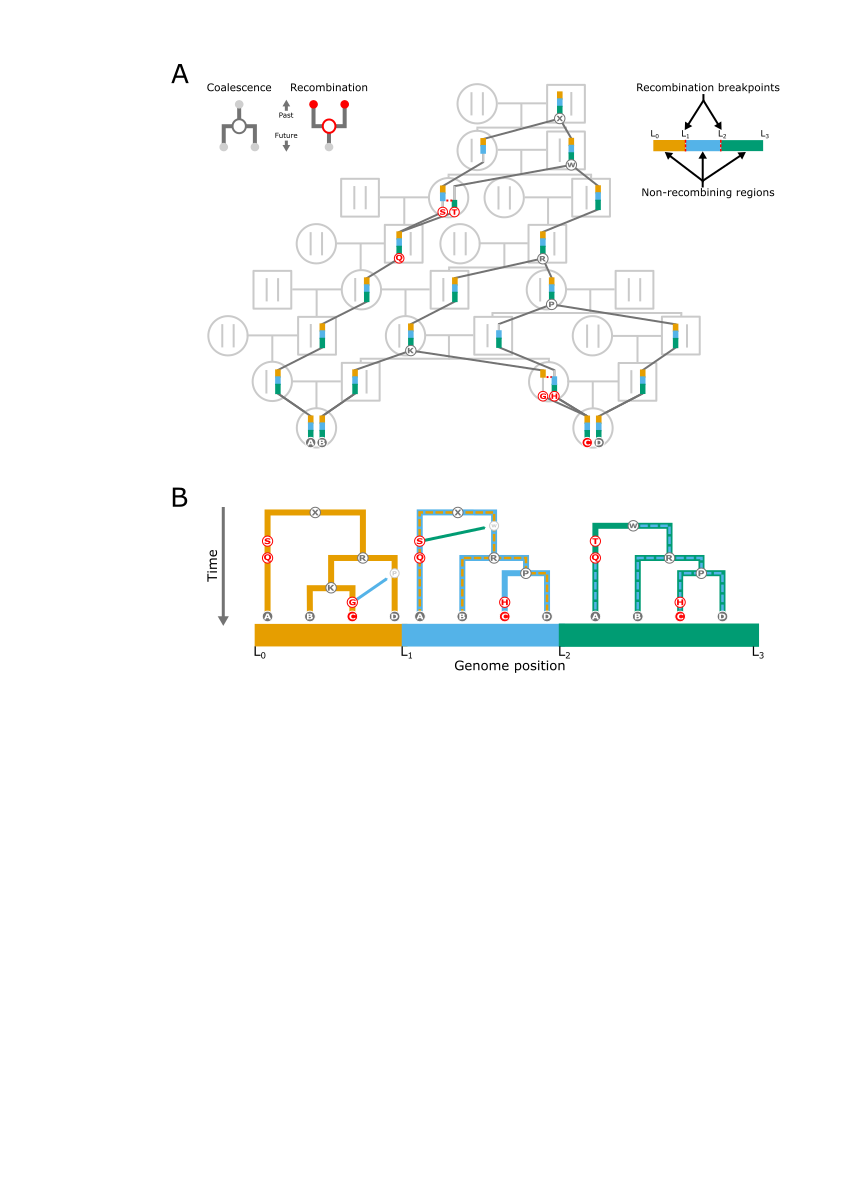
\includegraphics[width=\textwidth]{adapted_figs/arg_illustration.png}
    \caption[A simple example of an \acf{ARG}]{\textbf{A simple example of an \acf{ARG}}. (\textbf{A}) An \ac{ARG} (dark grey) embedded in a pedigree (light grey). Each node of the pedigree corresponds to an individual organism, connected by edges representing parent-offspring relationships. Each node of the \ac{ARG} corresponds to a haploid genome, connected by edges representing genetic inheritance between an ancestor and a descendant. Note that the example here assumes the samples are from the nuclear genome of sexually-reproducing diploid organisms, which is the most common scenario of interest. (\textbf{B}) An alternative representation of the \ac{ARG} in (\textbf{A}) as a series of local genealogies that share nodes and edges. The arrows represent \acf{SPR} operations associated with recombination events that convert local genealogies to their rightward neighbor. The dashed lines highlight each tree's shared structure with its leftward neighbor. Figure adapted from \cite{lewanski2023era} under a \href{https://creativecommons.org/licenses/by/4.0/}{CC BY 4.0} license.}
    \label{fig:intro-F1}
\end{figure}

Bifurcating nodes in an \ac{ARG} represent two types of events -- coalescence and recombination. A node where two edges enter from the future but only a single edge exit to the past represents when two lineages find common ancestry and \textit{coalesce} into a single lineage backward in time (e.g. grey coalescence nodes \textcircled{K}, \textcircled{P}, \textcircled{R}, \textcircled{W} and \textcircled{X} in Fig. \ref{fig:intro-F1}). Forward in time, a coalescence event occurs through a parent providing the same copy of genomic segment to multiple descendants. Conversely, a node where a single edge enter from the future but two edges exit to the past represents a single lineage of a \textit{recombinant} offspring from two parental lineages (e.g. red recombination nodes \textcircled{C} and \textcircled{Q} in Fig. \ref{fig:intro-F1}). Forward in time, a recombination node corresponds to a parent passing on a haploid gamete resulting from recombination between its two haploid genomes.

% talk about tree representation
The \ac{ARG} additionally records the age of each node (not labeled in Fig. \ref{fig:intro-F1}) as well as the position of the recombination breakpoint (dashed red lines in Fig. \ref{fig:intro-F1}) associated with each recombination node. Therefore, the full genealogy of every non-recombining genomic region can be constructed by traversing the the \ac{ARG} backwards in time and following the lineage on the appropriate side of the recombination breakpoint. The correspondence between the full \ac{ARG} and local genealogies naturally leads to an equivalent representation of an \ac{ARG} as a series of genealogical trees along the genome with shared nodes and edges (Fig. \ref{fig:intro-F1}B). Each local tree encodes the evolutionary history of a non-recombining genomic segment and can be transformed into the next one by removing a single edge and attaching it to a different node (arrows in Fig. \ref{fig:intro-F1}B). This operation termed \acf{SPR} reflects the outcome of a recombination event manifested in local genealogies. The graphical representation of a full \ac{ARG} can be recovered by sequentially combining the shared nodes and edges of each local tree while annotating each recombination node with its breakpoint position. In practice, the tree-sequence form of the \ac{ARG} (see \ref{intro-sim}) is frequently used both as the output of inference algorithms and input for downstream applications (\cite{lewanski2023era}), due to not only its tractability, but also the spatially local nature of many population genetic inference problems (such as identifying sites or region under selection).

%% Utilities of ARGs, give some examples of how problems can be formulated as questions about the ARG, mention sum stats
The \ac{ARG} constitutes the complete record of ancestral information among a set of genomes. Evolutionary processes such as selection, drift and gene flow all have a direct impact on the structure of an \ac{ARG}. Consequently, many population and evolutionary genetic questions can be formulated as inquiries into the \ac{ARG} (\cite{rasmussen_genome-wide_2014,lewanski2023era}). For example, the rate of coalescence reflected by the \ac{ARG} is informative of the effective population size over time, whereas the distribution of recombination breakpoints in the \ac{ARG} is directly tied to recombination rate across the genome. Furthermore, under the infinite sites model, samples of genomic sequences are stochastic readout of the \ac{ARG} through a Poisson process of mutations (\cite{wakeley2005coalescent}). Thus, any quantity or statistic derived from the genomic sequences (e.g. the \acs{SFS}, $F_{\mathrm{ST}}$, $\pi$, $\theta$, heterozygosity etc.) is but a low-dimensional summary of the underlying \ac{ARG} (\cite{ralph2020efficiently}). While these summary statistics have demonstrated great utility in providing meaningful evolutionary insights, the \ac{ARG} holds much richer information that can be tapped into for evolutionary analyses.

%% ARG inference methods

Although the \ac{ARG} is a powerful theoretical and conceptual tool to crack the code of evolution, in practice it must be inferred from population genomic data. \ac{ARG} inference has historically been a very challenging problem (\cite{rasmussen_genome-wide_2014,mathieson_what_2020}). The search space of all possible structures of an \ac{ARG} grows rapidly with increasing genome and sample sizes. In addition, as mentioned previously, the observed genomic sequences are noisy readout of the true \ac{ARG}. Mutation creates concordant patterns of genetic variation from which \acp{ARG} can be inferred, whereas recombination breaks up such patterns and reduces the amount of information per genealogy. The opposing forces of mutation and recombination impose a limit on \ac{ARG} identifiability from genomic sequences (\cite{hubisz2020inference,hayman2023recoverability}), which in turn limits the utility of \acp{ARG} in downstream applications. Early methods aimed to built a parsimonious \ac{ARG} that contains the minimal number of recombination events given a genotypic matrix (\cite{wong2023general}), which is a NP-hard problem (\cite{wang2001perfect}). These methods therefore rely on heuristics and are limited in scale of their applications. Recently, there has been great stride towards accurate \ac{ARG} inference at a practical scale. ARGweaver (\cite{rasmussen_genome-wide_2014}) and its extension ARGweaver-D (\cite{hubisz_mapping_2020}) mark the inception of statistically rigorous genome-wide \ac{ARG} inference. ARGweaver introduces a novel technique termed “threading” which adds an $n$-th sequence to an existing \ac{ARG} of $n-1$ sequences under a likelihood model defined by \iac{HMM}. The state space of the \ac{HMM} is simplified using approximations of the coalescent and discrete time to make the ``threading" operation a computationally tractable sampling step from the posterior distribution of \acp{ARG} using \ac{MCMC}. ARGweaver can be applied to up to a hundred whole genomes and remains the state of the art in terms of accuracy (\cite{brandt2022evaluation}). With the rapid growth of modern biobank-scale genomic datasets, a number of methods that balances statistical rigor and computational efficiency have been developed, such as Relate (\cite{speidel_method_2019}) and tsinfer/tsdate (\cite{kelleher_inferring_2019,wohns_unified_nodate}). These methods employ various heuristics and simplifications and consequently tend to underestimate recombination and only provide point estimates of the \ac{ARG} (\cite{lewanski2023era,wong2023general}), but have the remarkable ability to scale up to tens or even hundreds of thousands of genomic samples (see \cite{brandt2022evaluation} for a benchmark and comparison of prevailing inference methods). The suite of \ac{ARG} inference tools with a spectrum of accuracy-scalibility tradeoffs has paved the way for a new generation of methods that tackle a variety of empirical questions in population genetics (\cite{stern_approximate_2019,stern_disentangling_2021,speidel_method_2019}).

\section{Population-genetic simulations power large-scale \textit{in silico} experiments of evolution} \label{intro-sim}

%% Types of simulations: fwd vs. coal -> hybrid/ recapitation, accelerate
Without the ability to rewind time, we cannot observe evolution occur in real time in natural populations (barring some rare exceptions of feasible large-scale experimental evolutionary studies in species with short generation times). In most cases, \textit{in silico} simulations provide the only way to replay various evolutionary scenarios and conduct experiments of evolution. Population simulators are therefore an indispensable tool across all aspects of population genetic research ranging from validating theoretical expectations, testing hypothesis to powering Monte Carlo methods.

The process of simulating the evolution of a population may seem straightforward. We can simulate the reproduction of every individual in the population according to some model of choice, most commonly the Wright-Fisher model (\cite{wakeley2005coalescent,hahn2018molecular}). The simulation runs forward in time for many generations while mutation and recombination processes are recorded in the genomes of extant individuals at each generation. In the end, to generate one simulated dataset, some number of individuals and their genomes are sampled from the latest generation. This \textit{forward} simulation approach can be very flexible since it is facile to incorporate a wide range of evolutionary processes such as different forms of natural selection, complex demographic history or migration patterns into the simulations (\cite{hahn2018molecular}). However, forward simulations can become unwieldy in practice. First, since each individual needs to be tracked every generation, the amount of computation scales with the population size $N_e$, which is not uncommon to be quite large. In addition, simulations need to run until the population reaches equilibrium, which usually takes a number of generations on the order of the long-term $N_e$ (\cite{wakeley2005coalescent}). Hence, forward simulations scale approximately quadratically with the population size.

Researchers have come up with two types of techniques to circumvent the computational challenge. At its heart, population genomic simulations are simulations of the \ac{ARG} (see \ref{intro-arg}). Given a particular mutation model, neutral genetic variations in the genome are strictly governed by the \ac{ARG} (\cite{wakeley2005coalescent,hahn2018molecular}). Therefore, it is not necessary to generate neutral mutations during forward simulation. They can be overlaid onto the genealogies under a mutation model of choice to generate genomic sequences post hoc. The forward simulator SLiM (\cite{haller_slim_2019}) employs this tree-sequence recording procedure (\cite{haller_tree-sequence_2019}, also see below) to improve computational efficiency. Another key observation of the forward simulation process is that many historical individuals do not turn out to be genetic ancestors to the contemporary population from which the samples are taken. Therefore, if we take a \textit{backwards}-in-time approach, start from a sample of contemporary individuals and generate only the ancestors of these samples, we can avoid the computational burden of keeping track of the entire population every generation. This can be accomplished by sampling ancestral lineages under the coalescent process (\cite{kingman1982coalescent,kingman1982genealogy,hudson_gene_1990,tajima1983evolutionary}). The coalescent is an approximation of a forward Wright-Fisher population under the key assumption $N_e >> n$, where $N_e$ is the effective population size and $n$ the sample size. This assumption holds for many realistic use cases and therefore coalescent simulators provide a highly efficient way to generate population samples at scale. Coalescent simulations trade flexibility for computational efficiency. Early coalescent simulators were limited to only neutrally evolving populations (\cite{hahn2018molecular,lewanski2023era}). However, a new generation of coalescent simulators have emerged with the ability to handle more complex demographic scenarios and some form of selection. Among these, discoal (\cite{kern_discoal_2016}) and msprime (\cite{kelleher2016efficient}) have been most widely adopted to simulate biologically realistic samples at a practical scale.

A key innovation that has further revolutionized evolutionary simulations is the introduction of a \textit{hybrid} approach that exploits the strengths of both forward and backward (coalescent) simulators. The overall idea is to perform the more complex portion of the simulation where biological realism is paramount (e.g. population under various modes of selection) with a forward simulator and leave the simpler or less important portion (e.g. neutrally evolving population) to a coalescent simulator. This can be accomplished through either ``recapitation" of uncoalesced lineages in the first generation of a forward simulation until \iac{MRCA} is found with a coalescent simulator (\cite{haller_slim_2019}), or using a complete coalescent simulation to initialize a population and carry on the simulation with a forward simulator. This approach has been popularized thanks to the tskit python API (\cite{kelleher2016efficient,kelleher2018efficient}), which provides an interoperable data structure (ts format) for the tree-sequence encoding of the \ac{ARG}. The ts format is flexible, has a low storage footprint, and therefore has fostered an ecosystem of software tools along the simulation, inference and analysis pipeline of population genetic research.

Finally, it is worth mentioning that a community-driven effort to maintain a catalog of simulation models and a high-level API to simulate under these models out-of-the-box has emerged (\cite{adrion_community-maintained_2020,lauterbur_expanding_2022}). The stdpopsim project has made efficient large-scale simulations of complex evolutionary scenarios ever more accessible. The advancement of the simulation infrastructure has ultimately opened up opening up new opportunities and avenues for population genetic research, such as using simulations to generate perfectly labeled training data for supervised machine learning models.

\section{\ac{AI}/\ac{ML} methods for biomedical sciences}

\section{Studies of selective sweeps generate key insights into adaptive evolution}

\section{Objectives and outline of thesis}
